并行内核最基本的形式适用于基本的并行操作(例如:可以完全独立地、以任何顺序应用于每一块数据的操作)。通过使用这个形式,可以实现对调度的控制。因此,其是一个描述性编程结构的例子——调度决策由实现做出。\par

基本的数据并行内核是用单程序多数据(Single Program, Multiple Data, SPMD)风格编写的——“程序”(内核)应用于多段数据。注意,由于依赖于数据的分支,这个编程模型仍然允许内核在代码中采取不同的方式书写。\par

SPMD编程模型的最大优点,允许同一个“程序”映射到多个级别和类型的并行性,而无需提供任何指示。同一个程序的实例可以流水线化、打包在一起并使用SIMD指令执行、跨多个线程分布,或者混合使用这三种方法。\par

\hspace*{\fill} \par %插入空行
\textbf{理解数据并行内核}

并行内核的执行空间称为执行范围,内核的每个实例称为工作项。如图4-4所示。\par

\hspace*{\fill} \par %插入空行
图4-4 并行内核的执行空间,显示为2D范围内的64项
\begin{center}
	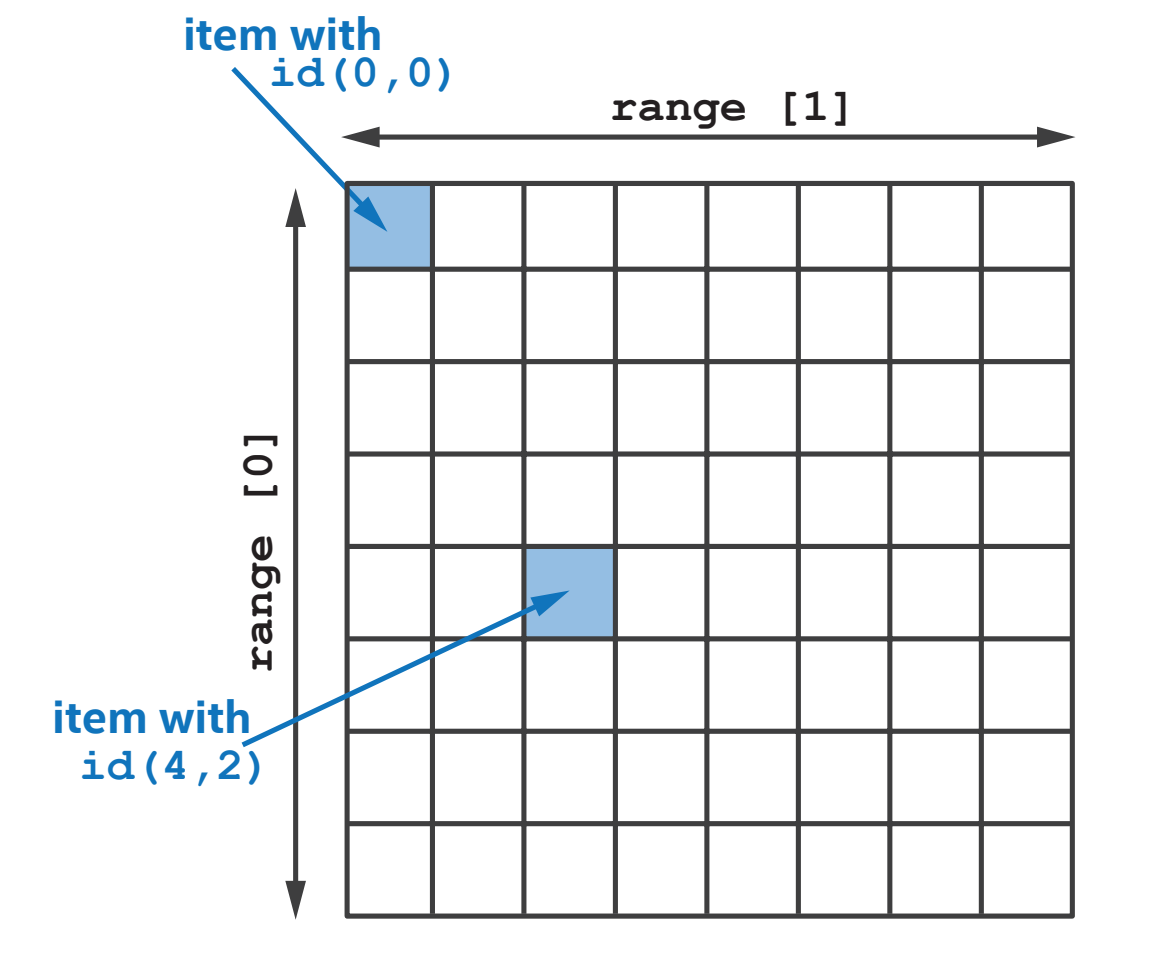
\includegraphics[width=1.\textwidth]{content/chapter-4/images/3}
\end{center}

数据并行内核的执行模型非常简单:允许完全并行执行。工作项可以以任何顺序执行,包括在单个硬件线程上顺序执行(即,没有任何并行性)!假设所有工作项都并行执行的内核(例如,尝试同步工作项),则很容易导致程序挂起。\par

为了保证正确性,必须假定内核可以并行执行。例如,确保对内存的并发访问可被原子操作保护(见第19章),以避免条件竞争。\par

\hspace*{\fill} \par %插入空行
\textbf{编写数据并行内核}

数据并行内核使用parallel\_for函数表示。图4-5展示了如何使用这个函数来表示向量加法。\par

\hspace*{\fill} \par %插入空行
图4-5 使用parallel\_for表示向量加法的内核代码
\begin{lstlisting}[caption={}]
h.parallel_for(range{N}, [=](id<1> idx) {
	c[idx] = a[idx] + b[idx];
});
\end{lstlisting}

该函数只接受两个参数:第一个参数是一个范围,指定在每个维度中启动工作项的数量,第二个参数是执行的内核函数。可以接受几个不同的类作为内核函数的参数,应该使用哪个类取决于该类公开所需的功能—稍后我们将继续讨论这个问题。\par

图4-6展示了一个非常类似的使用该函数来表示矩阵加法,(数学上)与向量加法相同,只是这次用于二维数据。这反映在内核中——两个代码片段之间的唯一区别是使用的范围和id类的维度!可以这样编码,因为SYCL访问器可以通过多维id进行索引。虽然看起来很奇怪,但非常强大,使我们能够编写基于数据维度的模板内核。\par

\hspace*{\fill} \par %插入空行
图4-6 用parallel\_for表示矩阵加法的内核代码
\begin{lstlisting}[caption={}]
h.parallel_for(range{N, M}, [=](id<2> idx) {
	c[idx] = a[idx] + b[idx];
});
\end{lstlisting}

C/C++中,使用多个索引和多个下标操作符为多维数据结构索引更为常见,访问器也支持这种显式索引。当内核同时操作不同维度的数据时,或者当内核的内存访问模式比直接使用项id描述的更复杂时,这种方式可以提高代码的可读性。\par

例如,图4-7中的矩阵乘法核必须提取索引的两个单独的分量,以便能够描述两个矩阵的行和列之间的点积。使用多个下标操作符(例如:[j][k])比混合多个索引模式和构造二维id对象(例如,id(j,k))更具可读性。\par

本章剩下的示例都使用了多个下标操作符,以确保访问的维度没有歧义。\par

\hspace*{\fill} \par %插入空行
图4-7 用parallel\_for表示方阵矩阵乘法的内核代码
\begin{lstlisting}[caption={}]
h.parallel_for(range{N, N}, [=](id<2> idx) {
	int j = idx[0];
	int i = idx[1];
	for (int k = 0; k < N; ++k) {
		c[j][i] += a[j][k] * b[k][i];
		// c[idx] += a[id(j,k) * b[id(k,i)]; <<< equivalent
	}
});
\end{lstlisting}

\hspace*{\fill} \par %插入空行
图4-8 将矩阵乘法映射到执行范围中的工作项上
\begin{center}
	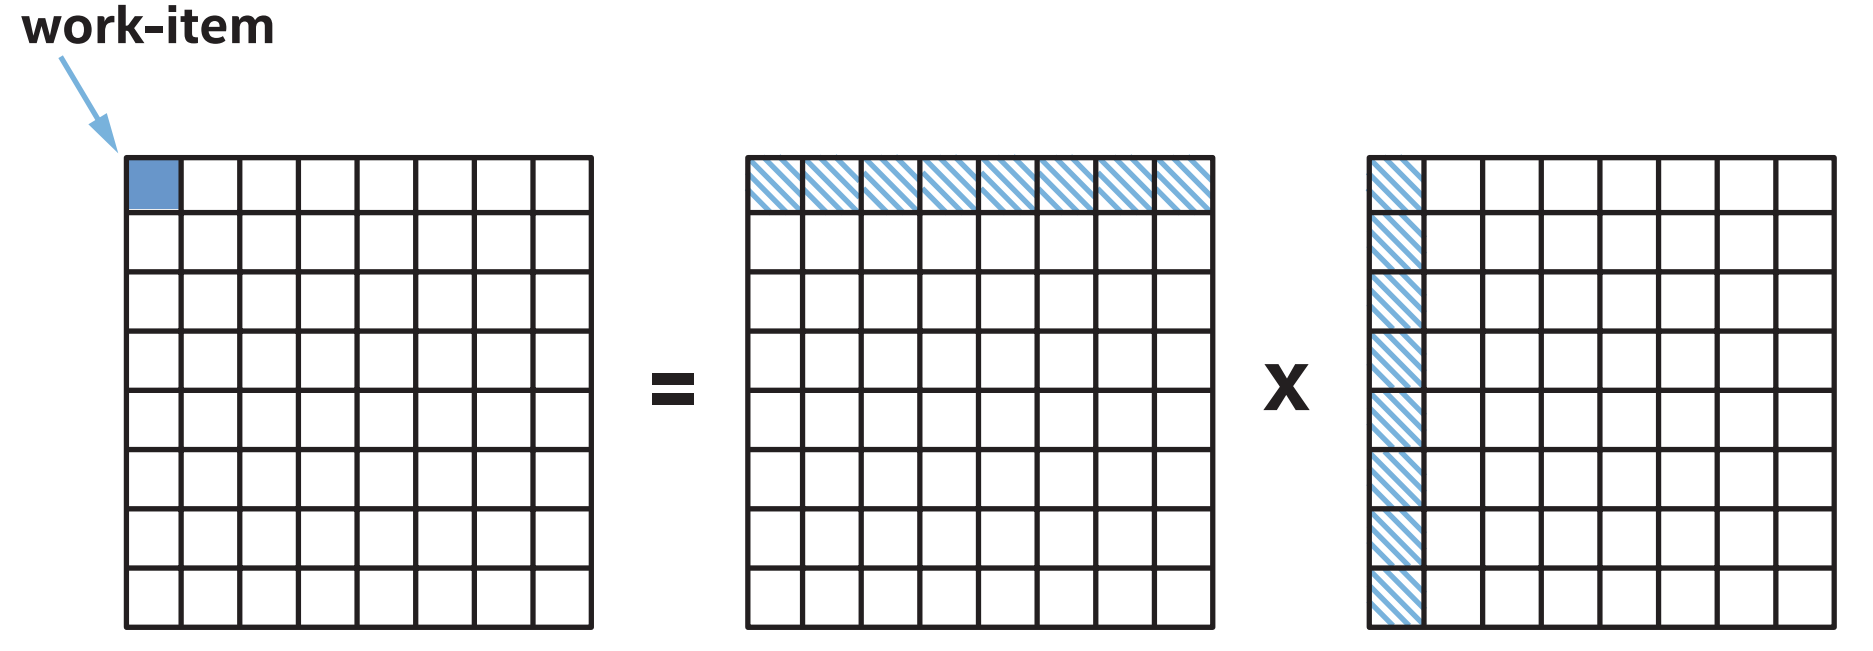
\includegraphics[width=1.\textwidth]{content/chapter-4/images/4}
\end{center}

图4-8中展示了如何将矩阵乘法内核中的工作映射到各个项。注意工作项的数量是来自输出范围的大小,多个工作项可能使用同样的输入值:每一个工作项计算C矩阵的一个值,通过顺序迭代A矩阵的行(连续的)和B(不连续)矩阵的列完成。\par

\hspace*{\fill} \par %插入空行
\textbf{数据并行内核的细节}

数据并行内核是通过三个C++类表示:range、id和item。前面的章节中,已经多次看到了range和id类,这里将以不同的重点继续讨论。\par

\hspace*{\fill} \par %插入空行
\textbf{range类}

range表示1、2或3维范围。range的维度是一个模板参数,必须在编译时已知,但每个维度的大小是动态的,并在运行时传递给构造函数。range类的实例用于描述并行执行范围和缓冲区的大小。\par

range类的简化定义显示了查询长度,构造函数和其他各种方法,如图4-9所示。\par

\hspace*{\fill} \par %插入空行
图4-9 简化的range类定义
\begin{lstlisting}[caption={}]
template <int Dimensions = 1>
class range {
public:
	// Construct a range with one, two or three dimensions
	range(size_t dim0);
	range(size_t dim0, size_t dim1);
	range(size_t dim0, size_t dim1, size_t dim2);
	
	// Return the size of the range in a specific dimension 
	size_t get(int dimension) const;
	size_t &operator[](int dimension);
	size_t operator[](int dimension) const;
	
	// Return the product of the size of each dimension
	size_t size() const;
	
	// Arithmetic operations on ranges are also supported
};
\end{lstlisting}

\hspace*{\fill} \par %插入空行
\textbf{id类}

id表示1、2或3维范围的索引。id的定义在许多方面与range相似:维数也必须在编译时已知,并且可以用于在索引内核的单个实例,或在缓冲区中创建偏移。\par

如图4-10中id类的简化定义所示,id在概念上只是包含1、2或3个整数的容器。可用的操作也非常简单:可以查询每个维度中索引,计算新的索引。\par

尽管可以构造id来表示任意索引,但要获得与特定内核实例关联的id,必须将它(或包含它的项)作为内核函数的参数。这个id(或它的成员函数返回的值)必须转发到任何想要查询索引的函数中——目前没有任何可以在程序中任意点查询索引的函数,但是这个问题DPC++会在未来来解决。\par

每个接受id的内核实例只知道分配给它计算的范围内的索引,而对range一无所知。如果想让内核实例知道自己的索引和范围,需要使用item类。\par

\hspace*{\fill} \par %插入空行
图4-10 简化的id类定义
\begin{lstlisting}[caption={}]
template <int Dimensions = 1>
class id {
public:
	// Construct an id with one, two or three dimensions
	id(size_t dim0);
	id(size_t dim0, size_t dim1);
	id(size_t dim0, size_t dim1, size_t dim2);
	
	// Return the component of the id in a specific dimension 
	size_t get(int dimension) const;
	size_t &operator[](int dimension);
	size_t operator[](int dimension) const;
	
	// Arithmetic operations on ids are also supported
};
\end{lstlisting}

\hspace*{\fill} \par %插入空行
\textbf{item类}

item表示内核函数的单个实例,封装了内核的执行range和实例在该range内的索引(分别使用一个range和一个id)。与range和id一样,维度必须在编译时就已知。\par

图4-11给出了工作项类的简化定义。item和id之间的主要区别是,item公开了额外的函数来查询执行范围的属性(例如:大小、偏移量)和一个计算线性化索引的函数。与id一样,获得与特定内核实例相关联的项的唯一方法是将它作为内核函数的参数。\par

\hspace*{\fill} \par %插入空行
图4-11 简化的item类定义
\begin{lstlisting}[caption={}]
template <int Dimensions = 1, bool WithOffset = true>
class item {
public:
	// Return the index of this item in the kernel's execution range
	id<Dimensions> get_id() const;
	size_t get_id(int dimension) const;
	size_t operator[](int dimension) const;
	
	// Return the execution range of the kernel executed by this item
	range<Dimensions> get_range() const;
	size_t get_range(int dimension) const;
	
	// Return the offset of this item (if with_offset == true)
	id<Dimensions> get_offset() const;
	
	// Return the linear index of this item
	// e.g. id(0) * range(1) * range(2) + id(1) * range(2) + id(2)
	size_t get_linear_id() const;
};
\end{lstlisting}










